% ****** Start of file apssamp.tex ******
%
%   This file is part of the APS files in the REVTeX 4.2 distribution.
%   Version 4.2a of REVTeX, December 2014
%
%   Copyright (c) 2014 The American Physical Society.
%
%   See the REVTeX 4 README file for restrictions and more information.
%
% TeX'ing this file requires that you have AMS-LaTeX 2.0 installed
% as well as the rest of the prerequisites for REVTeX 4.2
%
% See the REVTeX 4 README file
% It also requires running BibTeX. The commands are as follows:
%
%  1)  latex apssamp.tex
%  2)  bibtex apssamp
%  3)  latex apssamp.tex
%  4)  latex apssamp.tex
%
\documentclass[%
 reprint,
%superscriptaddress,
%groupedaddress,
%unsortedaddress,
%runinaddress,
%frontmatterverbose, 
%preprint,
%preprintnumbers,
%nofootinbib,
%nobibnotes,
%bibnotes,
 amsmath,amssymb,
 aps,
%pra,
%prb,
%rmp,
%prstab,
%prstper,
%floatfix,
]{revtex4-2}
\usepackage{multirow}
\usepackage{graphicx}% Include figure files
\usepackage{dcolumn}% Align table columns on decimal point
\usepackage{bm}% bold math
%\usepackage{hyperref}% add hypertext capabilities
%\usepackage[mathlines]{lineno}% Enable numbering of text and display math
%\linenumbers\relax % Commence numbering lines

%\usepackage[showframe,%Uncomment any one of the following lines to test 
%%scale=0.7, marginratio={1:1, 2:3}, ignoreall,% default settings
%%text={7in,10in},centering,
%%margin=1.5in,
%%total={6.5in,8.75in}, top=1.2in, left=0.9in, includefoot,
%%height=10in,a5paper,hmargin={3cm,0.8in},
%]{geometry}
\usepackage[utf8x]{inputenc} % Включаем поддержку UTF8  
\usepackage[russian]{babel}  % Включаем пакет для поддержки русского языка 
\usepackage[normalem]{ulem}  % для зачекивания текста

\begin{document}



\title{Лабораторная работа 5.5\\Компьютерная сцинтилляционная $\gamma$-спектропия}% Force line breaks with \\



\author{Батарин Егор Владиславович}
\affiliation{%
 Студент 3 курса РТ\\
 19 лет, скромный\\
 И просто хороший человек
}%

\collaboration{Московский физико-технический институт}%\noaffiliation

\date{6 сентября 2021 г.}% It is always \today, today,
             %  but any date may be explicitly specified
             

\begin{abstract}
Определяется энергия $\gamma$ - квантов неизвестного радиактивного препарата 
\begin{description}
\item[Оборудование]
Компьютер, сцинтиллятор, 5 образцов с радиоактивными материалами 
\end{description}
\end{abstract}

%\keywords{Suggested keywords}%Use showkeys class option if keyword
                              %display desired
\maketitle

%\tableofcontents

\section{Теоретическая часть.}
\subsection{Физика процессов, лежащих в основе лабораторной работы.}
	Основная задача спектрометрических измерений заключается в опреде-
лении энергии, интенсивности дискретных гамма-линий от различных гамма-
источников и их идентификации. В настоящее время используются различ-
ные типы гамма-детекторов: полупроводниковые, сцинтилляционные, пластиковые, жидкостные, газовые и т.д. Они существенно отличаются как по
своим спектрометрическим свойствам, так по эксплуатационным характеристикам и по технологии и стоимости изготовления.

В данной работе исследуются сцинтилляционные гамма-спектрометры на
основе неорганического кристалла NaI(Tl) и органической сцинтиллирующей
пластмассы.

Основными процессами взаимодействия гамма-излучения с веществом
являются фотоэффект, эффект Комптона и образо-
вание электрон-позитронных пар. Каждый из этих процессов вносит свой
вклад в образование наблюдаемого спектра.

\textbf{Фотоэффект} - процесс взаимодействия гамма-кванта с электроном, связанным с атомом, 
при котором электрону передается вся энергия гамма-кванта.

\textbf{Эффект Комптона} – упругое рассеяние фотона на свободном электроне,
сопровождающееся изменением длины волны фотона (реально этот процесс
происходит на слабо связанных с атомом внешних электронах). 

\textbf{Процесс образования электрон-позитронных пар.} При достаточно высокой энергии гамма-кванта наряду с фотоэффектом и эффектом Комптона
может происходить третий вид взаимодействия гамма-квантов с веществом –
образование электрон-позитронных пар. Процесс образования пар не может
происходить в пустоте, так как в этом случае не выполняются законы сохранения энергии и импульса. В присутствии ядра или электрона процесс образования пары гамма-квантом возможен, так как можно распределить энергию
и импульс гамма-кванта между тремя частицами без противоречия с законами сохранения. При этом если процесс образования пары идет в кулоновском
поле ядра или протона, то энергия образующегося ядра отдачи оказывается
весьма малой, так что пороговая энергия гамма-кванта, необходимая для
образования пары, практически совпадает с удвоенной энергией покоя электрона.

\subsection{Физика сцинтиллятора.}

При прохождении гамма-квантов через материальную среду образуются
электроны, возникающие за счет фотоэффекта, комптоновского рассеяния и
рождения электрон-позитронных пар. Образующиеся при этих процессах электроны испытывают большое количество неупругих соударений с молекулами и атомами
среды. Неупругие соударения могут сопровождаться как ионизацией, так и
возбуждением молекул или атомов среды. В промежуточных же стадиях (при
переходах возбужденных молекул или атомов в основное состояние, при
рекомбинации электрических зарядов и т.п.) в веществе возникают кван-
ты света различных длин волн, присущих данному веществу.

Вообще говоря, возникающее излучение должно сильно поглощаться в
сцинтилляторе, так как его энергия в точности равна энергии возбуждения
атомов среды. Чтобы избежать этого явления, в кристаллы сцинтиллятора
вводят небольшие добавки других атомов (в случае кристалла NaI это атомы
таллия). При этом спектр поглощения сдвигается относительно спектра
испускания в сторону меньших длин волн, и увеличивается вероятность
выхода из вещества хотя бы некоторой части квантов света, отвечающих
длинноволновому краю спектра испускания. В этом случае прохождение
ионизирующей частицы через вещество будет сопровождаться световой
вспышкой, которая и может быть использована для регистрации частицы.

Широкое применение сцинтилляционный метод исследования излучений
нашел после того, как были изобретены и усовершенствованы фотоэлектрон-
ные умножители (ФЭУ), позволяющие регистрировать весьма малые по дли-
тельности и очень слабые по интенсивности вспышки света. Таким образом,
современный сцинтилляционный счетчик состоит, в принципе, из сцинтилля-
тора — вещества, способного испускать видимое или ультрафиолетовое излу-
чение, возникающее под действием заряженных частиц, и фотоэлектронного
умножителя, в котором энергия этих световых вспышек через посредство
фотоэффекта преобразуется в импульсы электрического тока.

\subsection{Энергетическое разрешение спектрометра.}
Даже при поглощении часна выходе фотоприёмника
сцинтилляционного детектора меняется от события к событию. Это связано:

1) со статистическим характером процессов сбора фотонов на фотоприемнике и последующего усиления.

2) с различной вероятностью доставки фотона к фотоприёмнику из различных точке сцинтиллятора.

Энергетическим разрешением спектрометра называется величина

\begin{equation}
R_i = \frac{\Delta E_i}{E_i}
\end{equation}

где $\Delta E_i$ – ширина пика полного поглощения, измеренная на половине вы-
соты, $E_i$ – энергия регистрируемого гамма-излучения. Значение $E_i$ пропорцио-
нально среднему числу фотонов $n_i$ на выходе ФЭУ, т.е.:
\begin{equation}
E_i = \alpha\overline{n_i}
\end{equation}
Полуширина пика полного поглощения $\Delta E_i$ пропорциональна среднеквадратичной флуктуации $\overline{\Delta n_i}$. Так как $n_i$ - дискретная случайная величина, то  $\overline{\Delta n_i} = \sqrt{\overline{n_i}}$, значит 
\begin{equation}
\Delta E_i = \alpha\overline{\Delta n_i} = \alpha\sqrt{\overline{n_i}}	
\end{equation}

Из этих формул получаем:
\begin{equation}
R_i = \frac{\Delta E_i}{E_i} = \frac{\text{const}}{\sqrt{E_i}}
\end{equation}

\subsection{Схема установки.}

Принципиальная блок-схема гамма-спектрометра, изучаемого в данной
работе, показана на рисунке.

\begin{figure}[h!]
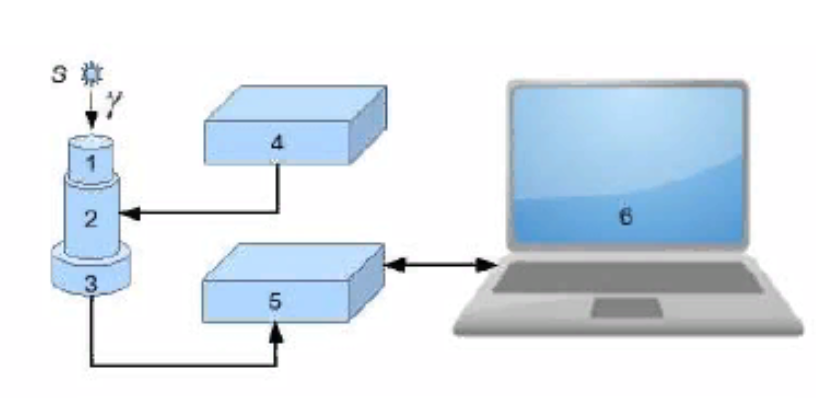
\includegraphics[scale=0.42]{1.png}
\end{figure}


На этом рисунке: 1 – сцинтиллятор, 2 – ФЭУ, 3 – предусилитель импуль-
сов,
4 – высоковольтный блок питания для ФЭУ, 5 – блок преобразования
аналоговых импульсов с ФЭУ в цифровой код (АЦП), 6 – компьютер для
сбора данных, их обработки и хранения.
ФЭУ со сцинтиллятором и блоком питания установлены на отдельной
подставке. В нашей работе на разных установках (стендах) в качестве сцин-
тиллятора используются кристаллы NaI(Tl) с размерами 45x50 мм и 
20x25 мм.

\section{Ход работы и обработка результатов.}

Прежде всего, исследуем, как "ползет" график в зависимости от ручки потенциометра:

\begin{figure}[h!]
	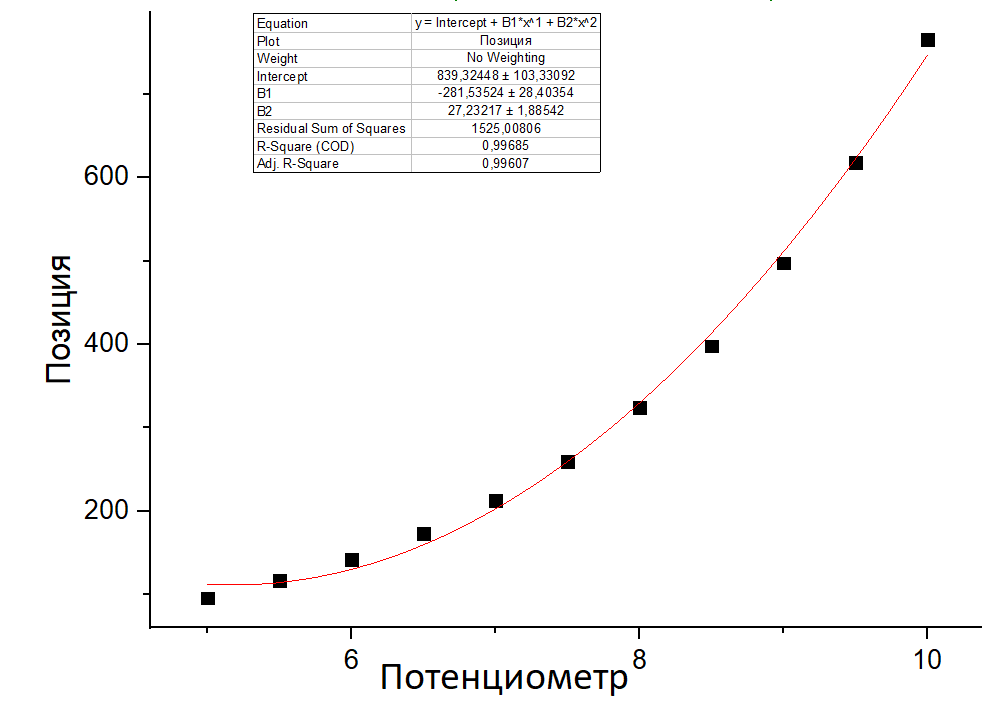
\includegraphics[scale=0.45]{2.png}
\end{figure}

Как видим, смещение графика в зависимости от поворота ручки потенциометра хорошо аппоксимируется квадратичной функцией. Самое маленькое значение потенциометра, на которое он был установлен, среди всех 5 образцов, равно $5.2$ - относительно этого значения будем проводить калибровку. В результате получаем таблицу:

\begin{table}[h!]
	\begin{tabular}{|l|l|l|}
		\hline
		Позиция & Значение кв. функции & Калибровка \\ \hline
		5,2     & 114                  & 0          \\ \hline
		5,4     & 115                  & 1          \\ \hline
		6,3     & 148                  & 34         \\ \hline
		9,5     & 617                  & 503        \\ \hline
		10      & 740                  & 626        \\ \hline
	\end{tabular}
\end{table}


Построим зависимость числа отсчетов $N$ от энергии $E$ и 4 дифференциальные кривые распределения энергии. Получаем:

=

\begin{figure*}[]
	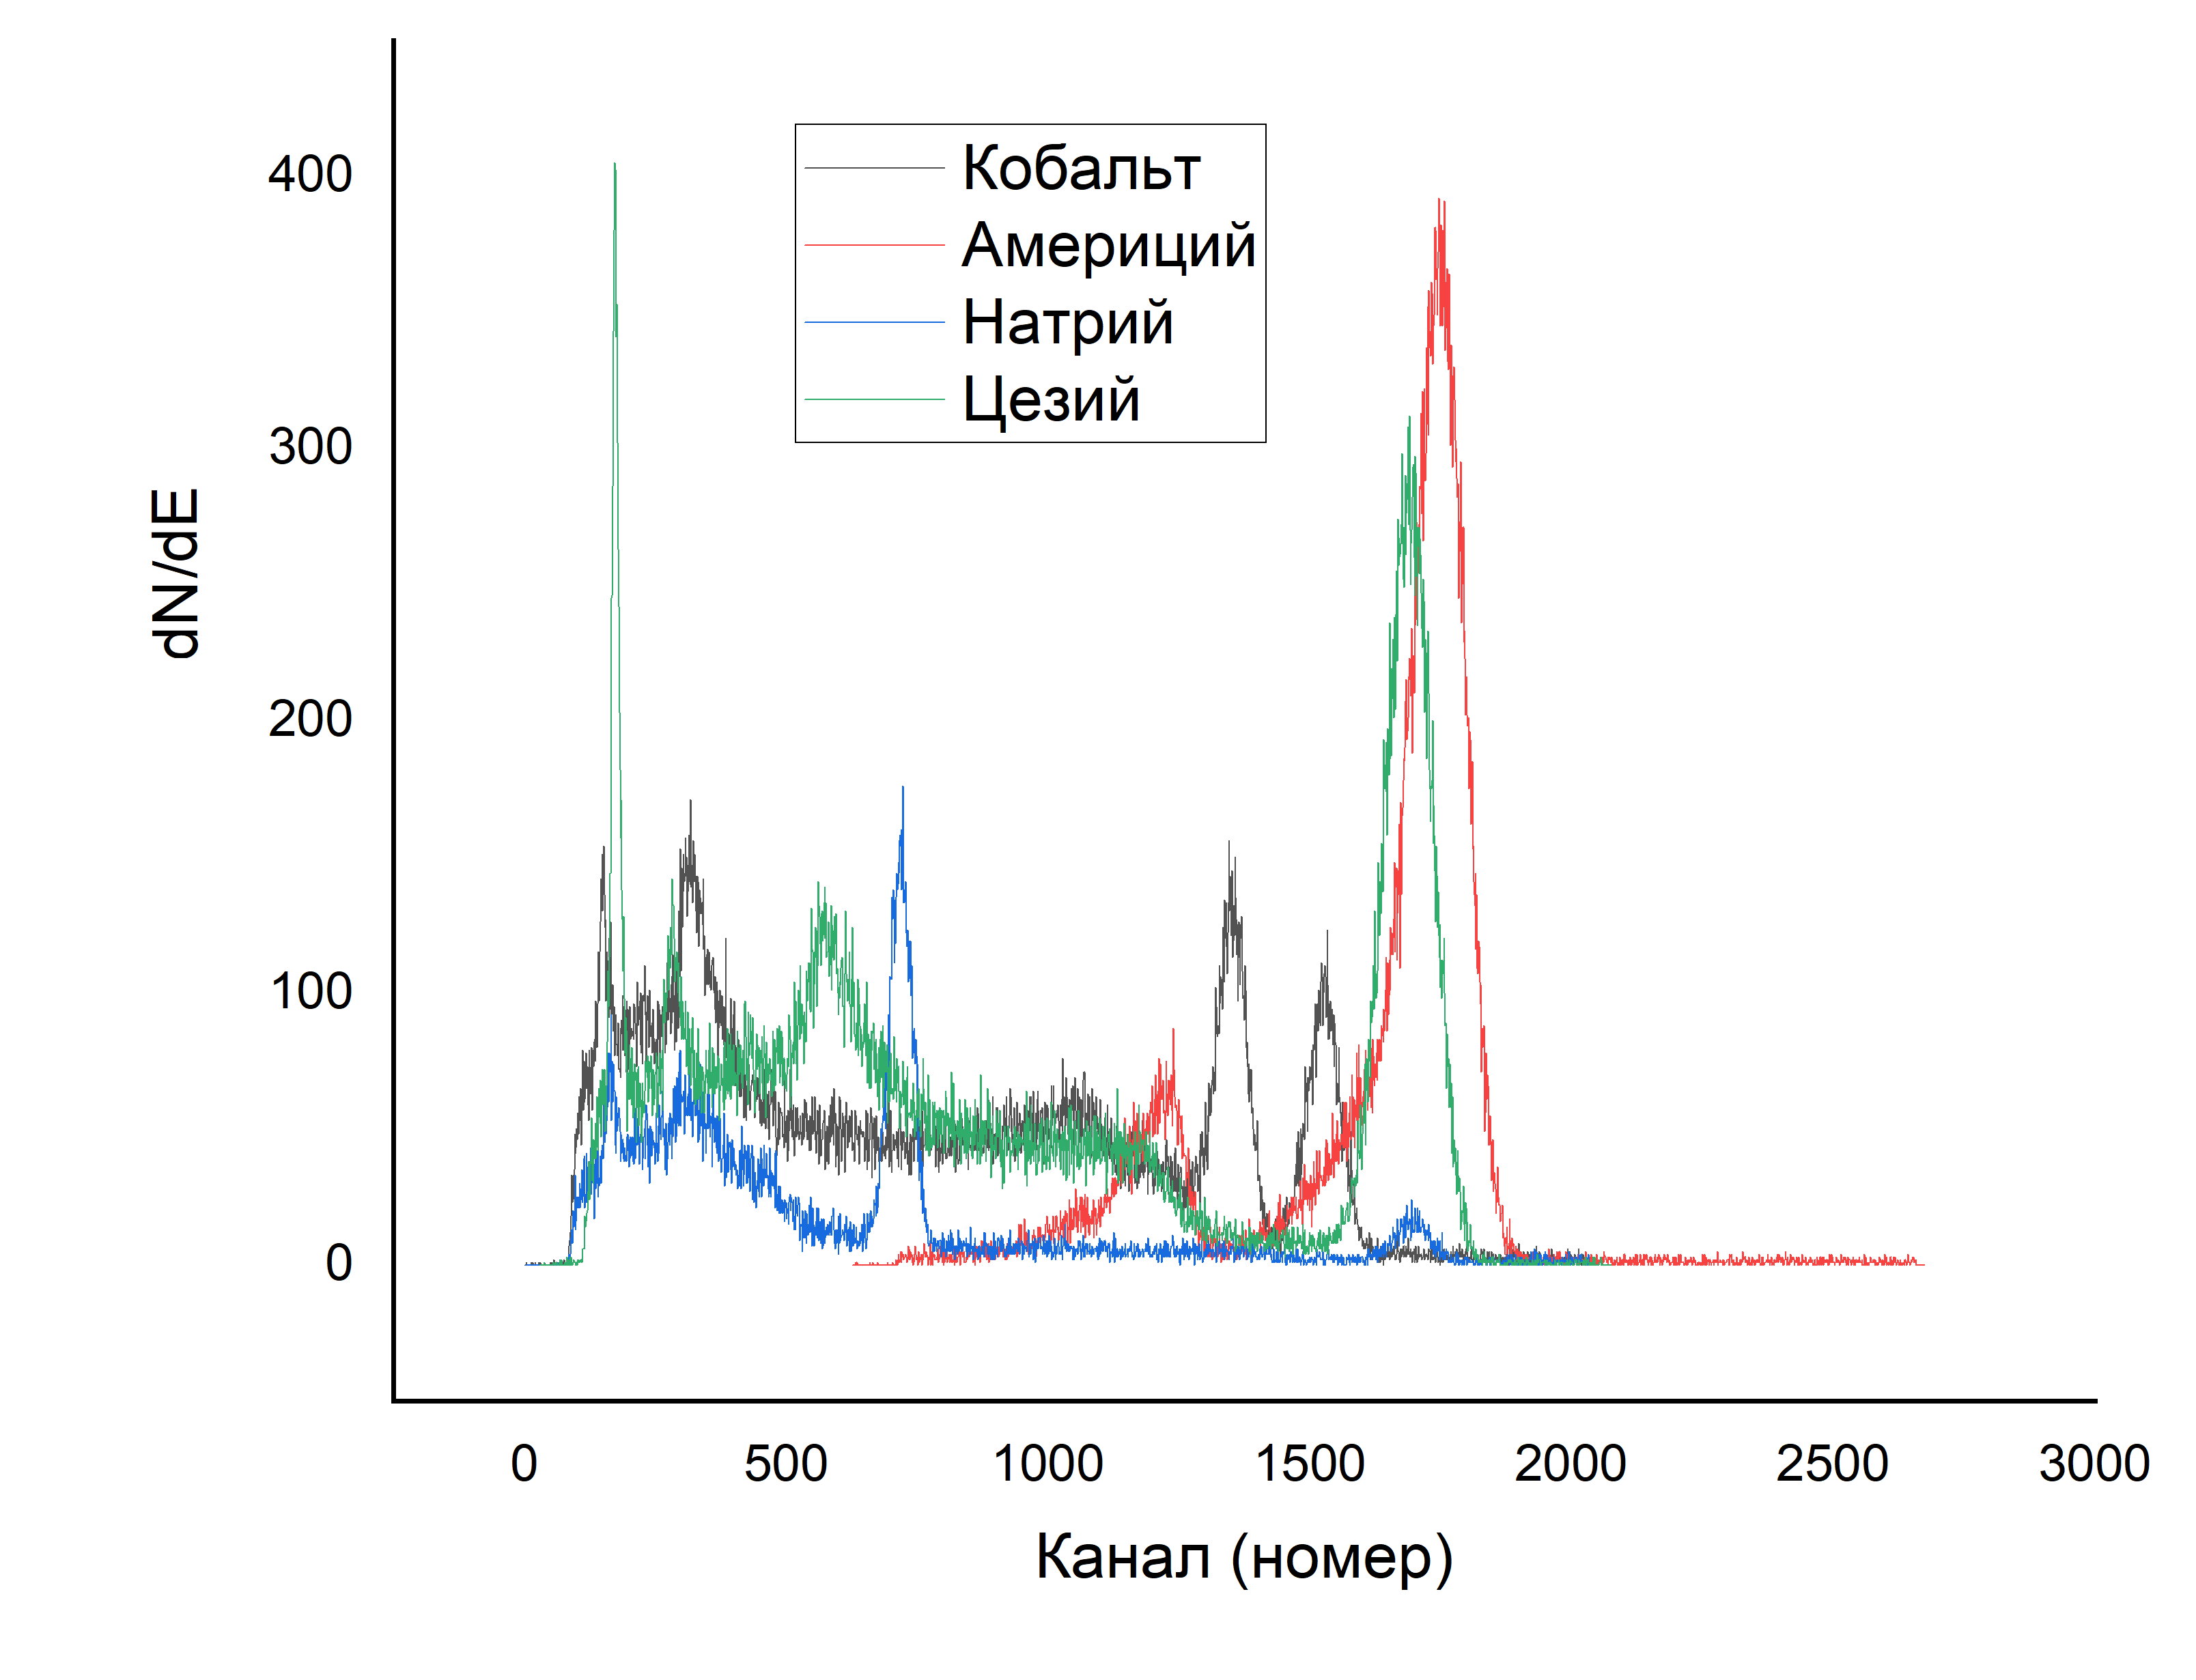
\includegraphics[scale=0.25]{3.png}
\end{figure*}


\begin{figure*}[]
	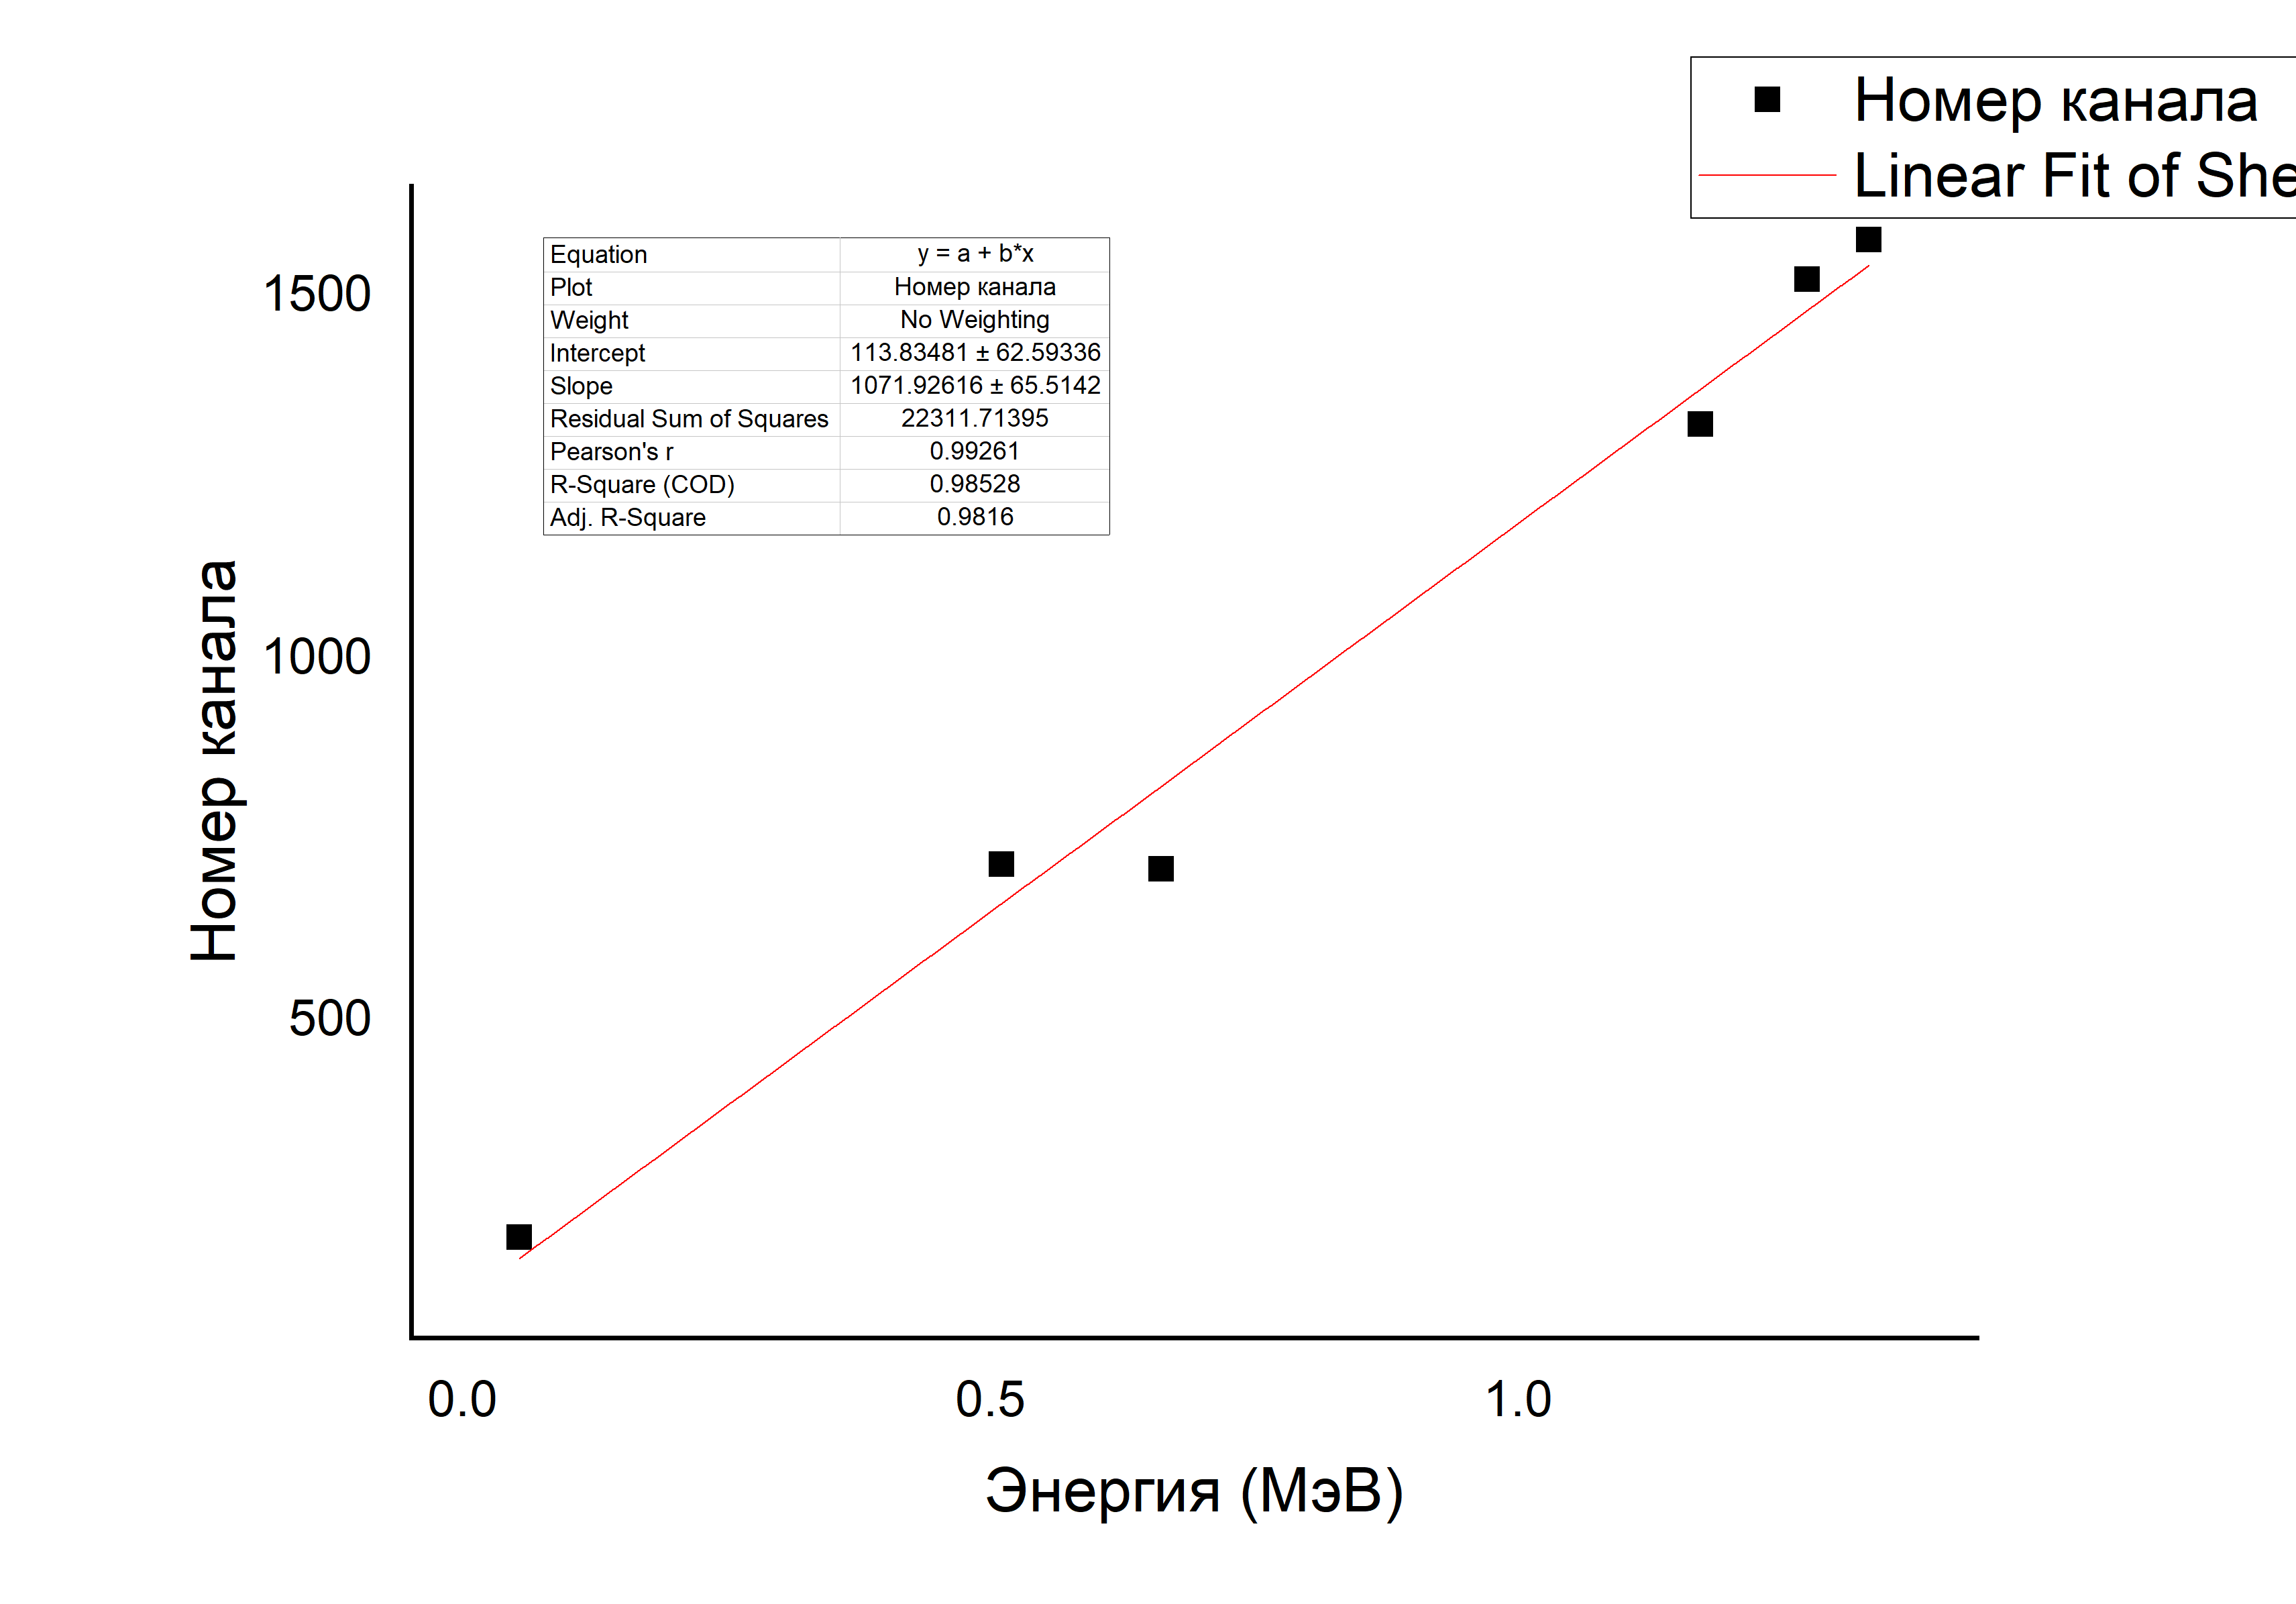
\includegraphics[scale=0.5]{4.png}
\end{figure*}



Для всех 4 образцов (полученный спектр Европия оказался слишком далеким от эталонного, потому был исключен из рассмотрения) получим следующую таблицу.

\begin{table}[]
	\begin{tabular}{|c|l|l|l|l|l|}
		\hline
		\multicolumn{1}{|l|}{Источник} & $N_i$  & $\Delta N_i$ & $E_i$, МэВ & $\Delta E_i$, МэВ & $R_i$     \\ \hline
		\multirow{2}{*}{Co-60}         & 1323  & 63.5                       & 1.1732    & 0.059235075                     & 0.05049  \\ \cline{2-6} 
		& 1578  & 72.4                       & 1.3325    & 0.067537313                     & 0.050685 \\ \hline
		\multirow{2}{*}{Na-22}         & 715.5 & 55.5                       & 0.511     & 0.051772388                     & 0.101316 \\ \cline{2-6} 
		& 1523  & 77.8                       & 1.274     & 0.072574627                     & 0.056966 \\ \hline
		Ce-137                         & 709   & 97.6                       & 0.6617    & 0.091044776                     & 0.137592 \\ \hline
		Am-241                         & 201   & 114                        & 0.054     & 0.106343284                     & 1.96932  \\ \hline
	\end{tabular}
\end{table}

Для всех данных, кроме Америция, проверим линейность зависимости $R^2 = f(1/E)$

\begin{figure*}[h!]
	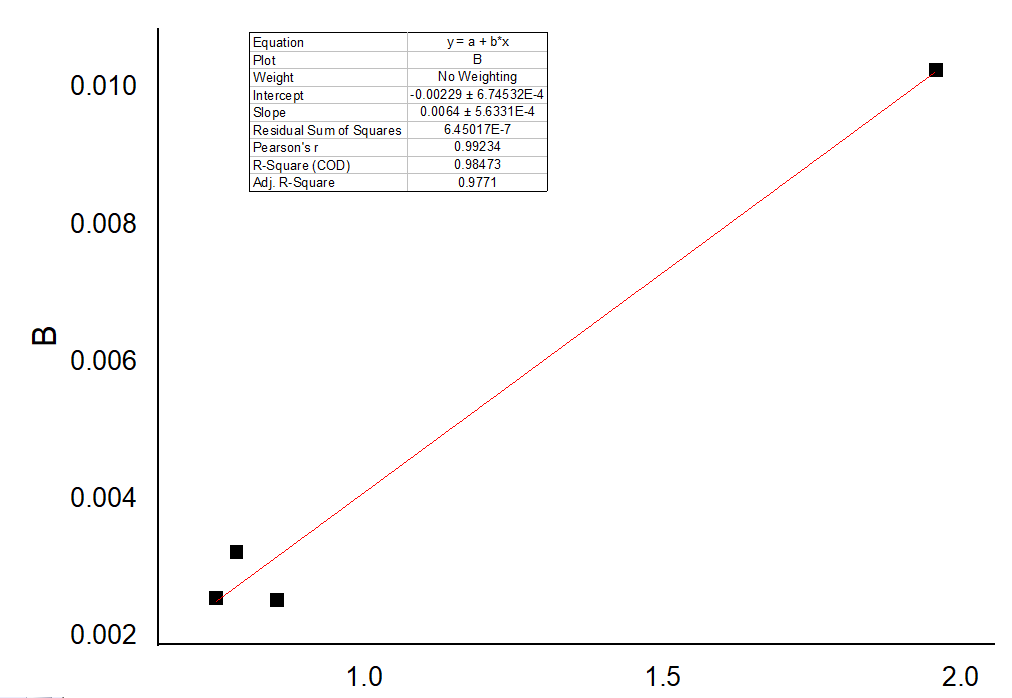
\includegraphics[scale=0.5]{5.png}
\end{figure*}
 Из графика можно заключить, что пик характеристического излучения свинца соответствует энергии примерно $300$ КэВ.

\end{document}
%
% ****** End of file apssamp.tex ******
